\begin{questions}
\question{
Eigenenergies and Spectrum
}
\begin{solution}.

  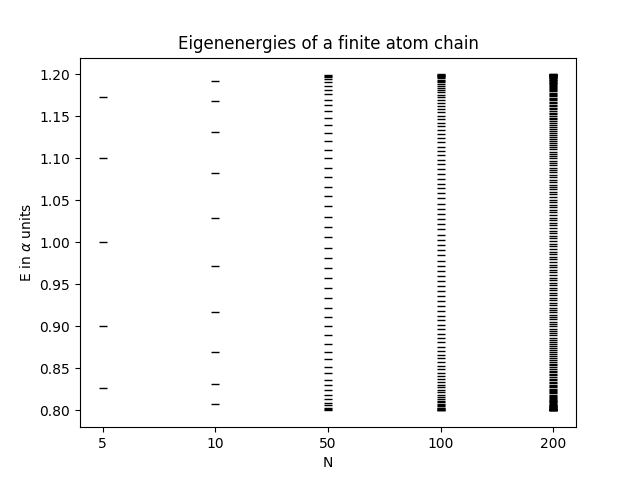
\includegraphics[width=80mm]{finite_chain.png}
  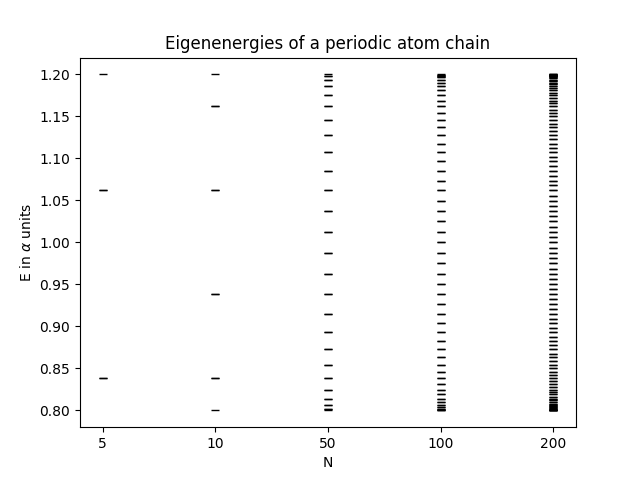
\includegraphics[width=80mm]{periodic_chain.png}\label{chain}

  \hspace{4cm}a)\hspace{7.7cm}b)

  \captionof{figure}{Eigenenergies of finite and periodic chain of atoms, a) and b) respectively. The $x$ axis denotes the number of atoms present in the chain and the $y$ axis shows the eigenenergies with in units of the on-site energy $\alpha$. Only interaction with nearest neighbours is considered, and the hopping is set to $\beta = 0.1\alpha$.}

 As in the lecture, we can see that as the number of atoms in the chain ($N$) increases the spectrum widens. Also we can see in both cases that when $N$ is too large the width of the spectrum is approximately $0.4$, this totally makes sense, since we expect the full width to be $4\beta$ when $N \rightarrow \infty$

 The spectrum of the finite chain is given by
 \begin{equation}
   E = \alpha + 2\beta\cos{(\pi m/(N+1))}, \quad m\in{1,\ldots,N}
   \label{fin:spec}
 \end{equation}
And as we can see in fig. \ref{fin:difs} the numericall results fit fairly well.

 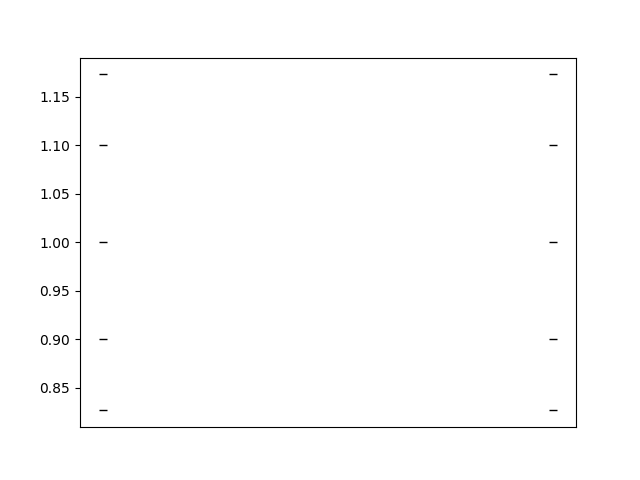
\includegraphics[width=80mm]{fin_comp.png}
 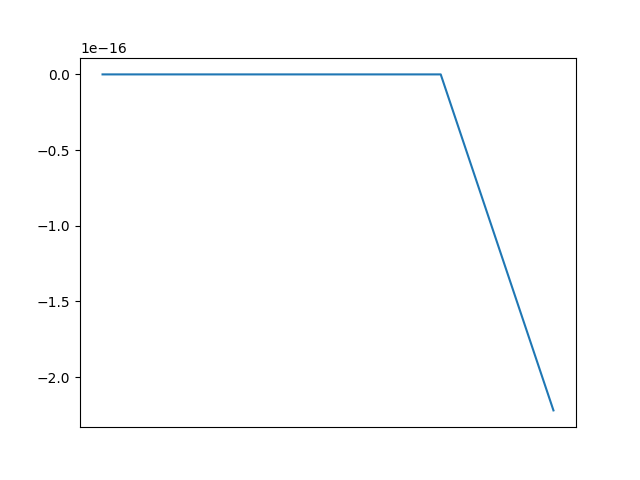
\includegraphics[width=80mm]{fin_dif_plot.png}\label{fin:difs}

 \hspace{4cm}a)\hspace{7.7cm}b)

 \captionof{figure}{a) On the left column the spectrum obtained numerically is shown, on the right the one obtained using eq. \ref{fin:spec}. b) The difference between the anallytical and the numerical spectrum is plotted. Both plots for the case when $N=5$, the remaining N values yield similar results.}

\end{solution}

\question{
Analysis of the periodic chain
}
\begin{solution}
  When we add periodic boundary conditions we can see that some degeneracies arise. Also we can see that no matter what N we have, we always have an energy of $1.2 = \alpha + 2\beta$, which is to be expected since the spectrum now is given by
  \begin{equation}
    E = \alpha + 2\beta\cos{(2\pi m/N)}, \quad m\in{0,1,\ldots,N-1},
    \label{spec}
  \end{equation}
  and $E = \alpha + 2\beta$ corresponds to the case when $m = 0$, which we always have. So, this is the reason why we can always reach that energy in the periodic chain as oposed to the finite chain. The degeneracies are explained by eq, \ref{spec} and the fact that the cosine is a periodic function. And finally, again as $N \rightarrow \infty$ the width of the spectrum tends to $4\beta$. As we can see on fig. \ref{per:difs}, the anallytical and numerical results for the spectrum fit also sufficiently well. Let's remember that $10^{-16}$ is the order of the machine error, so we can say that in both cases our approximations yielded sensible and trustable results.

  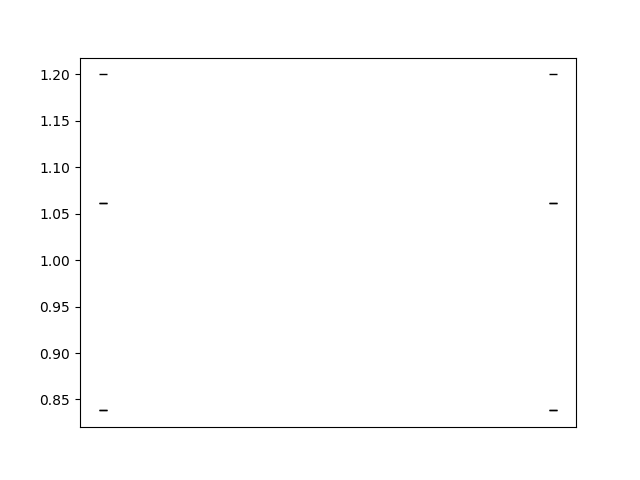
\includegraphics[width=80mm]{per_comp.png}
  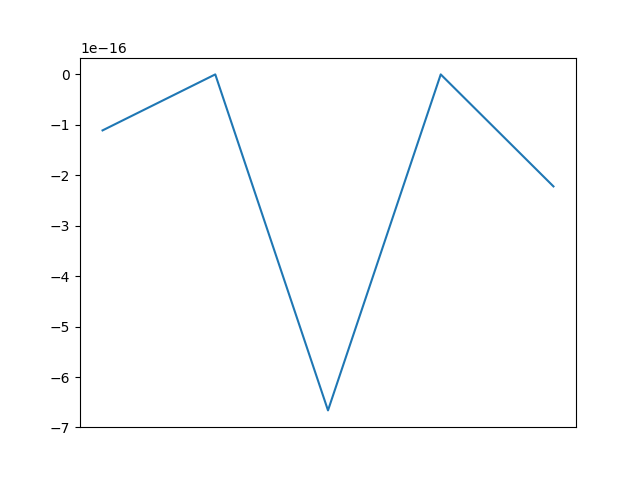
\includegraphics[width=80mm]{per_dif_plot.png}\label{per:difs}

  \hspace{4cm}a)\hspace{7.7cm}b)

  \captionof{figure}{Periodic chain case. a) On the left column the spectrum obtained numerically is shown, on the right the one obtained using eq. \ref{spec}. b) The difference between the anallytical and the numerical spectrum is plotted. Both plots for the case when $N=5$, the remaining N values yield similar results.}
\end{solution}
\end{questions}
